% THIS IS GDANSK UNIVERSITY OF TECHNLOGOGY (PG) PRESENTATION TEMPLATE
% Creator: Jan Cychnerski <jan.cychnerski@eti.pg.edu.pl>
% Copyleft 2019

% traditional screen
%\documentclass{beamer}

% wide screen
\documentclass[aspectratio=169]{beamer}


%%% YOUR PACKAGES HERE %%%
\usepackage{comment}
\usepackage{hyperref}
\usepackage{graphicx}
\usepackage{caption}


% polish language
\usepackage[polish]{babel}
\usepackage{polski}


%%% IMPORT PG PRESENTATION STYLE %%%
% THIS IS GDANSK UNIVERSITY OF TECHNLOGOGY (PG) PRESENTATION TEMPLATE
% Creator: Jan Cychnerski <jan.cychnerski@eti.pg.edu.pl>
% Copyleft 2019


% PG THEME OPTIONS

\usetheme{Boadilla}
\usecolortheme{default}
\usefonttheme{professionalfonts}

% colors

\definecolor{PGBlue}{RGB}{0,56,101}
\definecolor{PGRed}{RGB}{193,10,39}
\definecolor{PGSilver}{RGB}{200,200,200}
\definecolor{PGBlack}{RGB}{0,0,0}

% PGBlue
\setbeamercolor{frametitle}{fg=PGBlue}
\setbeamercolor{normal text}{fg=PGBlue}
\setbeamercolor{structure}{fg=PGBlue}
\setbeamercolor{item}{fg=PGBlue}

% PGRed
\setbeamercolor{alerted text}{fg=PGRed}
\setbeamercolor{item projected}{fg=PGRed}

% white
\setbeamercolor{title}{fg=white}
\setbeamercolor{titlelike}{fg=white}
\setbeamercolor{subtitle}{fg=white}

% enumerate and itemize styles

\setbeamertemplate{itemize item}{\bfseries\color{PGRed}\raise1pt\hbox{\donotcoloroutermaths$\bullet$}}
\setbeamertemplate{itemize subitem}{\color{PGRed}\raise0.5pt\hbox{--}}
\setbeamertemplate{itemize subsubitem}{\color{PGRed}\tiny\raise1.5pt\hbox{\donotcoloroutermaths$\bullet$}}

\setbeamertemplate{enumerate item}{\bfseries\color{PGRed}\insertenumlabel.}
\setbeamertemplate{enumerate subitem}{\color{PGRed}\insertsubenumlabel.}
\setbeamertemplate{enumerate subsubitem}{\color{PGRed}\insertsubsubenumlabel.}
\setbeamertemplate{enumerate mini template}{\insertenumlabel}


% disable navigation

\beamertemplatenavigationsymbolsempty

% additional commands

\newcommand*{\vcenteredhbox}[1]{\begingroup
\setbox0=\hbox{#1}\parbox{\wd0}{\box0}\endgroup}

\graphicspath{{pgbeamer/}}


\usepackage{iflang}
\IfLanguageName{polish}{
\newcommand{\pglogobig}{pg-logo-big-pl}
\newcommand{\pglogosmall}{pg-logo-small-pl}
}{
\newcommand{\pglogobig}{pg-logo-big-en}
\newcommand{\pglogosmall}{pg-logo-small-en}
}


% FRAME TITLE LOGO
\addtobeamertemplate{frametitle}{\vcenteredhbox{\includegraphics[height=8mm]{\pglogosmall}}\bfseries}{}


\newcommand{\pgtitleframe}{{
% PG TITLE PAGE

\setbeamercolor{background canvas}{bg=PGBlue}
\setbeamercolor{title}{fg=white}
\setbeamercolor*{date}{fg=white}
\setbeamercolor*{author}{fg=white}

\setbeamertemplate{footline}{}

\begin{frame}[noframenumbering]
\centering
\vspace{1cm}
\includegraphics[height=3cm]{\pglogobig}
\vspace{5mm}
\maketitle
\end{frame}
}}

\newcommand{\pglastframe}{{
% PG LAST PAGE

\setbeamercolor{background canvas}{bg=PGBlue}
\setbeamercolor{title}{fg=white}
\setbeamercolor*{date}{fg=white}
\setbeamercolor*{author}{fg=white}

\setbeamertemplate{footline}{}

\begin{frame}[noframenumbering]
\centering
\vspace{1cm}
\includegraphics[height=5cm]{\pglogobig}
\end{frame}
}}



%%% YOUR OPTIONS HERE %%%

\title[PG Presentation]{Licencjonowanie w sieciach komputerowych}
\author{inż. Mikołaj Nowak \and inż. Jakub Grzybowski \and inż. Wojciech Baranowski}
\date{\today}

%%% DOCUMENT BEGINS HERE %%%

\begin{document}

%%% PG TITLE PAGE %%%
\pgtitleframe

%%% YOUR PRESENTATION HERE %%%

\setbeamercovered{invisible}
\author{M. Nowak \and J. Grzybowski \and W. Baranowski}

\begin{frame}{Czym jest stos TCP/IP?}
  \begin{columns}
    \begin{column}{0.55\textwidth}
      \begin{itemize}
        \item Zestaw protokołów komunikacyjnych używanych w sieciach komputerowych.
        \item Obejmuje cztery główne warstwy:
        \begin{itemize}
          \item Aplikacji
          \item Transportową
          \item Internetową
          \item Dostępu do sieci
        \end{itemize}
        \item Jest zaimplementowany jako część jądra systemu operacyjnego.
        \item Umożliwia komunikację w Internecie i sieciach lokalnych.
      \end{itemize}
    \end{column}
    \begin{column}{0.4\textwidth}
      \centering
      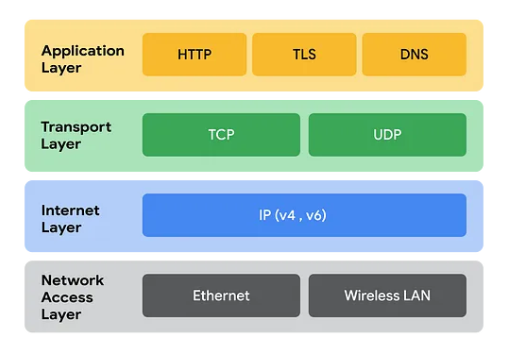
\includegraphics[width=\linewidth]{tcpip.png}
    \end{column}
  \end{columns}
\end{frame}

\begin{frame}{Rodzaje licencji oprogramowania}
  \begin{itemize}
    \item \textbf{Otwarte licencje (Open Source):}
    \begin{itemize}
      \item \textbf{GPL (GNU General Public License):} wymaga udostępnienia kodu źródłowego oraz wszelkich zmian – tzw. \textit{copyleft}.
      \item \textbf{BSD, MIT:} pozwalają na modyfikację i wykorzystanie komercyjne bez obowiązku udostępniania zmian.
    \end{itemize}
    \vspace{0.5em}
    \item \textbf{Zamknięte licencje (Proprietary):}
    \begin{itemize}
      \item Kod źródłowy nie jest publicznie dostępny.
      \item Brak możliwości legalnej modyfikacji i redystrybucji.
      \item Oprogramowanie objęte licencją końcowego użytkownika (\textit{EULA}).
    \end{itemize}
    \vspace{0.5em}
    \item Licencje wpływają na rozwój, bezpieczeństwo i elastyczność oprogramowania.
  \end{itemize}
\end{frame}

\begin{frame}{Znaczenie licencji dla stosu TCP/IP}
  \begin{itemize}
    \item Implementacja stosu TCP/IP jest zwykle częścią jądra systemu operacyjnego.
    \item Licencja jądra decyduje o:
    \begin{itemize}
      \item dostępie do kodu źródłowego stosu,
      \item możliwości modyfikacji i ponownego rozpowszechniania,
      \item integracji z innym oprogramowaniem (np. komercyjnym).
    \end{itemize}
    \vspace{0.5em}
    \item \textbf{Otwarte jądra} (np. Linux, BSD) pozwalają na:
    \begin{itemize}
      \item audyt bezpieczeństwa,
      \item eksperymenty naukowe i edukacyjne,
      \item tworzenie niestandardowych rozszerzeń.
    \end{itemize}
    \vspace{0.5em}
    \item \textbf{Zamknięte jądra} (np. Windows, iOS) ograniczają kontrolę nad działaniem sieci.
  \end{itemize}
\end{frame}

\begin{frame}{Linux}
  \begin{itemize}
    \item Jądro Linuxa jest licencjonowane na zasadach \textbf{GPLv2 (GNU General Public License)}.
    \item Stos TCP/IP jest jego integralną częścią – licencja obejmuje cały kod źródłowy.
    \item Użytkownicy mają pełen dostęp do kodu, mogą go:
    \begin{itemize}
      \item analizować,
      \item modyfikować,
      \item dystrybuować dalej (z zachowaniem GPL).
    \end{itemize}
    \item Bogate możliwości rozszerzania dzięki modułom takim jak:
    \begin{itemize}
      \item \texttt{netfilter}, \texttt{nftables} – filtrowanie pakietów,
      \item \texttt{eBPF} – dynamiczne programowanie zachowania stosu w jądrze.
    \end{itemize}
    \item Wykorzystywany w wielu środowiskach: od serwerów i komputerów po Androida i IoT.
  \end{itemize}
\end{frame}

\begin{frame}{macOS / iOS}
  \begin{itemize}
    \item Systemy Apple bazują na \textbf{Darwinie} – jądrze typu Unix, opartym częściowo na \textbf{FreeBSD}.
    \item Część komponentów (w tym fragmenty stosu TCP/IP) pochodzi z BSD i są dostępne na licencji \textbf{BSD}.
    \item Apple jednak wprowadza własne rozszerzenia i modyfikacje, które:
    \begin{itemize}
      \item nie są publicznie dostępne,
      \item objęte są licencjami zastrzeżonymi,
      \item mogą być zamknięte mimo otwartego „rdzenia”.
    \end{itemize}
    \item Oficjalna licencja źródłowego Darwina: \textbf{APSL (Apple Public Source License)} – niezgodna z GPL, uważana za problematyczną.
    \item Stos TCP/IP w macOS/iOS to więc:
    \begin{itemize}
      \item kombinacja komponentów BSD,
      \item zamkniętych rozszerzeń Apple,
      \item fragmentów o niejednoznacznym statusie licencyjnym.
    \end{itemize}
  \end{itemize}
\end{frame}

\begin{frame}{Windows}
  \begin{itemize}
    \item Systemy Windows korzystają z własnościowego stosu TCP/IP – zamkniętego i niedostępnego publicznie.
    \item Stos został zaimplementowany samodzielnie przez Microsoft – początkowo w Windows NT, dziś obecny we wszystkich wersjach.
    \item Brak dostępu do kodu źródłowego oznacza:
    \begin{itemize}
      \item brak możliwości modyfikacji lub audytu,
      \item pełną zależność od aktualizacji Microsoftu,
      \item niemożność dostosowania do nietypowych zastosowań.
    \end{itemize}
    \item Licencjonowanie odbywa się wraz z systemem – użytkownik akceptuje \textit{EULA}, bez wpływu na wewnętrzne komponenty.
    \item Dla programistów dostępne są tylko wysokopoziomowe API (np. WinSock), ale nie kod źródłowy implementacji.
  \end{itemize}
\end{frame}

\begin{frame}{BSD (FreeBSD / OpenBSD / NetBSD)}
  \begin{itemize}
    \item Rodzina systemów BSD korzysta z licencji \textbf{BSD} – bardziej liberalnej niż GPL.
    \item Licencja pozwala na:
    \begin{itemize}
      \item modyfikację i dowolne wykorzystanie kodu,
      \item zamknięcie kodu w produktach komercyjnych bez obowiązku publikacji zmian.
    \end{itemize}
    \item \textbf{FreeBSD} – popularny w serwerach i systemach NAS (np. TrueNAS).
    \item \textbf{OpenBSD} – znany z nacisku na bezpieczeństwo i audyt kodu.
    \item \textbf{NetBSD} – ekstremalnie przenośny, działa na setkach architektur.
    \item Kod stosu TCP/IP z BSD jest wykorzystywany m.in. w:
    \begin{itemize}
      \item MacOS i iOS (częściowo)
      \item Juniper JunOS,
      \item Sony PlayStation.
    \end{itemize}
  \end{itemize}
\end{frame}

\begin{frame}{RouterOS / VxWorks / Cisco IOS}
  \begin{itemize}
    \item Systemy te są ściśle powiązane ze sprzętem i mają wbudowany, zamknięty stos TCP/IP.
    \item \textbf{RouterOS (MikroTik):}
    \begin{itemize}
      \item oparty częściowo na Linuksie, ale całość zamknięta,
      \item brak dostępu do kodu źródłowego,
      \item licencjonowany na zasadach komercyjnych – wg klucza lub poziomu.
    \end{itemize}
    \item \textbf{Cisco IOS:}
    \begin{itemize}
      \item zamknięty system operacyjny dla routerów i przełączników Cisco,
      \item zintegrowany stos TCP/IP, brak możliwości modyfikacji,
      \item licencja przypisana do urządzenia (hardware-locked).
    \end{itemize}
    \item Wspólną cechą jest:
    \begin{itemize}
      \item brak otwartości i modyfikowalności,
      \item pełna kontrola producenta nad aktualizacjami i funkcjami.
    \end{itemize}
  \end{itemize}
\end{frame}

\begin{frame}{Porównanie podejścia systemów operacyjnych}
\scriptsize
\begin{tabular}{|p{2.5cm}|p{2cm}|p{2.3cm}|p{2.2cm}|p{4.0cm}|}
  \hline
  \textbf{System operacyjny} & \textbf{Kod źródłowy} & \textbf{Licencja} & \textbf{Modyfikowalność} & \textbf{Typowe zastosowanie} \\
  \hline
  Linux & Tak & GPLv2 & Pełna & Serwery, IoT, Android \\
  \hline
  macOS iOS & Częściowo & Mieszana & Ograniczona & Komputery i urządzenia Apple \\
  \hline
  Windows & Nie & Komercyjna & Brak & Komputery osobiste, środowiska korporacyjne \\
  \hline
  FreeBSD OpenBSD NetBSD & Tak & BSD & Pełna & Routery, OS-y wbudowane, \mbox{macOS} (pośrednio) \\
  \hline
  RouterOS Cisco IOS VxWorks & Nie & Komercyjna sprzętowa & Brak & Routery, urządzenia sieciowe, systemy embedded \\
  \hline
\end{tabular}
\note{Zestawienie pozwala porównać otwartość kodu i praktyczne konsekwencje w kontekście TCP/IP.}
\end{frame}

\begin{frame}{Lekkie stosy TCP/IP – lwIP, uIP}
  \begin{itemize}
    \item Niektóre zastosowania (IoT, mikrokontrolery, embedded) wymagają lekkich implementacji stosu TCP/IP.
    \item \textbf{lwIP (lightweight IP):}
    \begin{itemize}
      \item Licencja BSD – pełna dowolność wykorzystania,
      \item zoptymalizowany pod wydajność i niskie zużycie zasobów,
      \item używany w systemach z ograniczoną pamięcią (np. ESP32, STM32).
    \end{itemize}
    \item \textbf{uIP (micro IP):}
    \begin{itemize}
      \item Jeszcze mniejszy niż lwIP – działa na urządzeniach z <64KB RAM,
      \item zintegrowany z systemem Contiki (IoT, sensory),
      \item podstawowe wsparcie dla TCP, UDP, ICMP.
    \end{itemize}
    \item Oba stosy są często używane w środowiskach, gdzie pełny OS byłby zbyt ciężki.
  \end{itemize}
\end{frame}

\begin{frame}{Podsumowanie i wnioski}
  \begin{itemize}
    \item \textbf{Licencja ma realny wpływ} na to, jak stos TCP/IP może być używany, rozwijany i modyfikowany.
    \item \textbf{Otwarte systemy} (Linux, BSD):
    \begin{itemize}
      \item umożliwiają pełny dostęp do stosu TCP/IP,
      \item wspierają eksperymenty, badania i rozwój,
      \item promują transparentność i bezpieczeństwo.
    \end{itemize}
    \item \textbf{Zamknięte systemy} (Windows, macOS, RouterOS):
    \begin{itemize}
      \item ograniczają kontrolę użytkownika,
      \item wymagają zaufania do producenta,
      \item są trudne lub niemożliwe do audytu.
    \end{itemize}
    \item Wybór systemu to wybór między elastycznością a wygodą (i czasem – wsparciem komercyjnym).
  \end{itemize}
\end{frame}

\begin{frame}{Kryptografia w sieciach komputerowych}
  Sieci komputerowe dzisiaj nieodzownie łączą się z kryptografią, która pozwala nam zapewnić atrybuty bezpieczeństwa informacji takie jak: poufność, integralność, uwierzytelnianie i niezaprzeczalność. Nie zawsze tak jednak było... 
\end{frame}

\begin{frame}{Historia eksportu kryptografii z USA}
  \begin{itemize}
      \item Podczas zimnej wojny istniały silne regulacje ograniczające eksport technologii krytycznej z USA do Bloku Wschodniego, do której zaliczana była kryptografia
      \item Eksportem zarządzała organizacja CoCom (Coordinating Committee for Multilateral Export Controls)
      \item W latach 60 organizacje finansowe zaczynały zgłaszać zapotrzebowanie na opracowanie rozwiązań kryptograficznych celem zabezpieczenia rozwijających się przelewów elektronicznych
  \end{itemize}
\end{frame}

\begin{frame}{Data Encryption Standard - DES}
    \begin{itemize}
      \item Na początku lat 70 NIST (National Institute of Standards and Technology) zdecydowało się na wprowadzenie rządowego standardu szyfrowania.
      \item IBM w odpowiedzi na zapotrzebowanie zaproponowało swój standard - znany później jako DES
      \item Oryginalny DES zakładał wykorzystanie kluczy 128-bitowych, NSA (National Security Agency) nalegało na skrócenie długości do 48 bitów. Jako "kompromis" zastosowano klucze 56-bitowe.
      \item Ponadto NSA wprowadziło zmiany do algorytmu, których uzasadnienie nie zostało podane do wiadomości publicznej. Pojawiły się spekulacje o wprowadzenie tylnich drzwi
      \item DES został opublikowany w 1977 jako standard federalny FIPS PUB 46
    \end{itemize}
\end{frame}

\begin{frame}{Rivest–Shamir–Adleman Cryptosystem - RSA}
    \begin{itemize}
        \item W 1977 trójka naukowców opracowała algorytm RSA
        \item Próba opublikowania algorytmu mogłaby skutkować karą więzienia dla autorów
        \item Algorytmy kryptograficzne z punktu widzenia prawa traktowane były jak broń
        \item Dokument opisujący RSA był kopiowany i przekazywany pocztą pantoflową
        \item Rząd USA ugiął się i pozwolił na publikację pracy w 1979
        \item W 1983 algorytm został opatentowany (w USA). Patent wygasł w roku 2000.
    \end{itemize}
\end{frame}

\begin{frame}{Pretty Good Privacy - PGP}
    \begin{itemize}
        \item W 1991 Phil Zimmerman stworzył program PGP umożliwiający szyfrowanie oraz cyfrowe podpisywanie tekstu, maili, plików, katalogów a nawet całych partycji dyskowych
        \item Było to jedno z pierwszych narzędzi które umożliwiały każdemu stosowanie algorytmów kryptograficznych
        \item Opublikowany w domenie publicznej (public domain)
        \item Oprogramowanie trafiło też poza USA
        \item Rząd stanów zjednoczonych rozpoczął śledztwo przeciwko Zimmermanowi pod kątem nielicencjonowanego eksportu broni
        \item Wówczas wszystkie systemy kryptograficzne używające ponad 40 bitów były uważane za broń. PGP używało kluczy 128-bitowych
    \end{itemize}
\end{frame}

\begin{frame}{PGP - naruszenie patentu RSA}
    \begin{itemize}
        \item Zimmerman naruszył także patent który od 1983 obejmował RSA.
        \item Organizacja, która zarządzała patentem na RSA zażądała od Zimmermana zaprzestania dystrybucji PGP
        \item Sam Zimmerman faktycznie zaprzestał... 
        \item Co dało odwrotny efekt - oprogramowanie jeszcze bardziej zyskało na popularności i ludzie jeszcze chętniej je rozpowszechniali
    \end{itemize}
\end{frame}

\begin{frame}{PGP - pierwsze zastosowania i obawy}
    \begin{itemize}
        \item PGP świetnie sprawdziło się u ludzi żyjących w krajach rządzonych przez opresyjne rządy
        \item NSA argumentowało, że oprogramowanie będzie używane przez pedofili i przestępców
        \item W praktyce takie argumenty można zastosować do wielu innych wynalazków
    \end{itemize}
\end{frame}

\begin{frame}{PGP vs USA - ciąg dalszy}
    \begin{itemize}
        \item Rząd USA naciskał na konieczność wdrażania tylnych drzwi dla służb przez firmy tworzące oprogramowanie
        \item Administracja Billa Clintona powiedziała kongresowi "Americans have no Constitutional right to choose their own method of encryption"
        \item Ludzie zwracali uwagę na podobieństwo kodu i innych form wolności słowa
        \item Zimmerman przekonał MIT do wydrukowania kodu, oprawienia go w książkę i wysłania do europejskich bibliotek
        \item Rząd wiedział, że gdyby zablokowali wydanie książki, skutkowałoby to sprawą sądową którą by przegrał ze względu na naruszenie pierwszej poprawki (wolność religii, słowa, prasy, zgromadzeń i petycji)
        \item Stosowano też inne, niecodzienne formy eksportu
    \end{itemize}
\end{frame}

\begin{frame}{Eksport kryptografii - obejścia}
    \begin{figure}
        \centering
        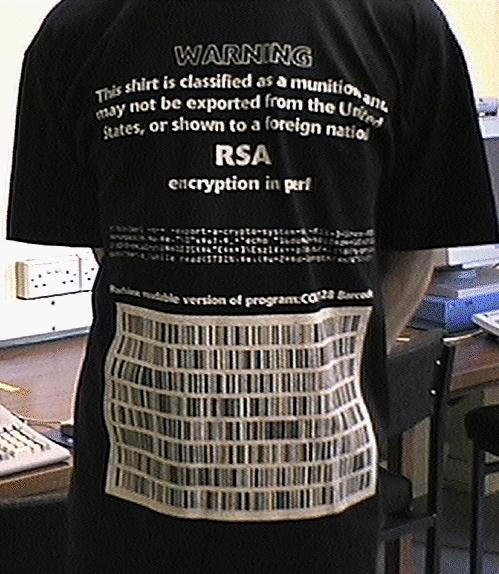
\includegraphics[width=0.5\linewidth]{lo-main/rsa.jpg}
    \end{figure}
\end{frame}

\begin{frame}{Eksport kryptografii - obejścia}
    \begin{figure}
        \centering
        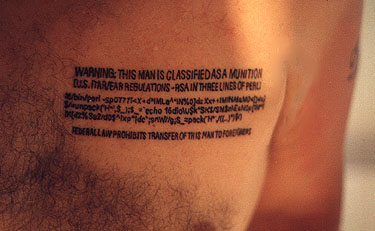
\includegraphics[width=0.75\linewidth]{lo-main/rsa2.jpg}
    \end{figure}
\end{frame}

\begin{frame}{Eksport kryptografii - obejścia}
    \begin{figure}
        \centering
        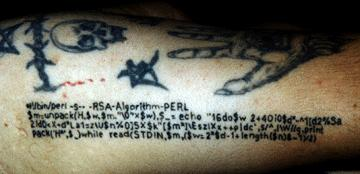
\includegraphics[width=0.8\linewidth]{lo-main/rsa3.jpg}
    \end{figure}
\end{frame}

\begin{frame}{PGP vs USA - ciąg dalszy}
    \begin{itemize}
        \item Sąd po przeanalizowaniu sprawy Zimmermana uznał, że oprogramowanie szyfrujące jest chronione przez pierwszą poprawkę i nie powinno się ograniczać jego rozpowszechniania
        \item Wszelkie akcje prawne przeciwko Zimmermanowi zostały wstrzymane
        \item Do dnia dzisiejszego rządy nie są zadowolone z kryptografii i często naciskają na producentów oprogramowania na wprowadzanie do oprogramowania tylnej furtki
    \end{itemize}
\end{frame}

\begin{frame}{PGP dziś}
    \begin{itemize}
        \item PGP zostało przejęte przez firmę Network Associates Inc. (NAI) i przekształciło się w rozwiązanie komercyjne
        \item Oprócz rozwiązania komercyjnego powstał też otwarty standard OpenPGP
        \item Najbardziej znaną implementacją standardu OpenPGP jest GnuPG (GPG), działającą w latach 1997-2007 na licencji GPL-2.0-or-later a od 2007 na licencji GPL-3.0-or-later
        \item GPG nie może używać opatentowanych algorytmów, PGP (komercyjne) może używać tych, na które wykupiło licencje
        \item Jako że patenty działają w obrębie danego kraju, istnieją wtyczki umożliwiające GPG korzystanie z algorytmów zastrzeżonych np. w USA. Oczywiście nie powinny być one stosowane przez mieszkańców USA.
    \end{itemize}
\end{frame}

\begin{frame}{Inne rozwiązania}
    Do innych rozwiązań kryptograficznych działających w sieciach komputerowych możemy zaliczyć:
    \begin{itemize}
        \item OpenSSL - wieloplatformowa implementacja protokołów SSL i TLS i innych algorytmów kryptograficznych. Wcześniej udostępniana była na licencji OpenSSL License / SSLeay license, zbliżonej do licencji Apache, od wersji 3.0 wydanej w 2018 roku obowiązuje licencja Apache-2.0
        \item OpenVPN - oprogramowanie do tworzenia sieci VPN udostępniane na licencji GPLv2
        \item WireGuard - oprogramowanie do tworzenia VPN, nowsze, prostsze i szybsze niż OpenVPN, licencje różnią się w zależności od implementacji (MIT/Apache 2.0/GPLv2/GPLv3)
        \item OpenSSH - oprogramowanie bazujące na protokole SSH umożliwiające zestawienie bezpiecznego połączenia w niezabezpieczonej sieci. Udostępnione na licencji BSD.
    \end{itemize}
\end{frame}

\begin{frame}{Bibliografia}
    \begin{itemize}
        \item Thomas R. Johnson "American Cryptology during the Cold War, 1945-1989.Book III: Retrenchment and Reform, 1972-1980"
        \item Film dokumentalny "Cypherpunks Write Code" produkcji magazynu Reason
        \item philzimmermann.com
        \item Stallings, W.: Cryptography and network security: principles and practice.
    \end{itemize}
\end{frame}

%%% PG LAST PAGE %%%
\pglastframe

%%% DOCUMENT ENDS HERE. Good bye! :) %%%

\end{document}
